\section{Shared Memory}

\frame{\frametitle{Index}\tableofcontents[currentsection]}

\begin{frame}
	\frametitle{OpenMP}
	\begin{block}{Implementation}
		\begin{itemize}
			\item AOS \& SOA;
			\item Similar to sequential version:
			\begin{itemize}
				\item \texttt{parallel for} added to both core functions;
			\end{itemize}
		\end{itemize}
	\end{block}

	\begin{block}{Load Balance}
		\begin{itemize}
			\item Core functions are homogeneous;
			\begin{itemize}
				\item [] (exception: \update, if number of edges per cell differs)
			\end{itemize}
			\item Static scheduling:
			\begin{itemize}
				\item Round-robin;
			\end{itemize}
		\end{itemize}
	\end{block}
\end{frame}

\begin{frame}
	\frametitle{Results}
	\begin{figure}
		\centering
		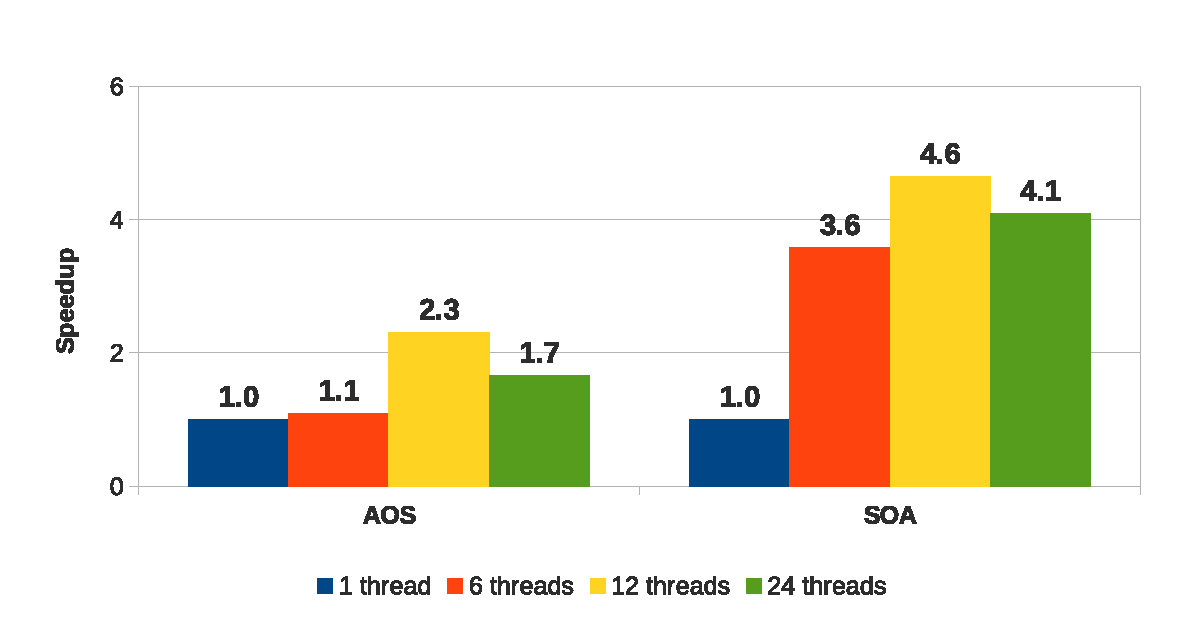
\includegraphics[width=\textwidth]{graph_comparison_omp.eps}
	\end{figure}
\end{frame}

\begin{frame}
	\frametitle{Limitations}
	\begin{itemize}
		\vfill
		\item Locality issues:
		\vfill
		\begin{itemize}
			\item Softened with SOA;
			\vfill
			\item Depends on the mesh structure;
			\begin{itemize}
				\item \texttt{gmsh} does not optimize the mesh;
			\end{itemize}
			\vfill
			\item Highly researched topic:
			\begin{itemize}
				\item Hoppe, 1999;
				\item Complex approach;
			\end{itemize}
			\vfill
			\item Specialized libraries:
			\begin{itemize}
				\item \texttt{parmetis};
				\item Unknown complexity;
			\end{itemize}
		\end{itemize}
	\end{itemize}
\end{frame}